% !TEX TS-program = xelatex
% !TEX encoding = UTF-8 Unicode
\documentclass[gap.tex]{subfiles}
\begin{document}
\label{sec:pilot-score}
Each pilot’s score is the sum of that pilot’s distance, time, leading and
arrival points, rounded to the nearest whole number, 0.5 being rounded up.
\[ \forall p : p \in PilotsLaunched : TotalScore_p = DistancePoints_p + TimePoints_p + LeadingPoints_p + ArrivalPoints_p \]
\subsection{Distance points}
\label{sec:distance-points}
The distance considered for each pilot to calculate distance points is that
pilot’s best distance along the course line, up until the pilot landed or the
task deadline was reached, whichever comes first.

\begin{hg}
One half of the available distance points are assigned to each pilot linearly,
based on the pilot’s distance flown in relation to the best distance flown in
the task. The other half is assigned taking into consideration the difficulty
of the kilometers flown.
\begin{align*}
    LinearFraction_p &= \frac{Distance_p}{2 * BestDistance} \\
    i_p &= \lfloor Distance_p * 10 \rfloor \\
    DifficultyFraction_p &= DiffScore_{i_p} + ((DiffScore_{i_{p + 1}} - DiffScore_{i_p}) * (Distance_p * 10 - i_p)) \\
    DistancePoints_p &= (LinearFraction_p + DifficultyFraction_p) * AvailableDistancePoints
\end{align*}
\end{hg}

\begin{pg}
In the case of a stopped task, a pilot’s distance may be increased by an
altitude bonus (see~\ref{sec:distance-stopped-tasks}). The available distance
points are assigned to each pilot linearly, based on the pilot’s distance flown
in relation to the best distance flown in the task.
\[ DistancePoints_p = \frac{Distance_p}{BestDistance} * AvailableDistancePoints \]
\end{pg}

\subsubsection{Difficulty calculation}
\label{sec:difficulty-calculation}
\begin{hg}
To measure the relative difficulty of each 100 meters of the task, we consider
the number of pilots who landed in the successive few kilometers, and the
distance flown.

In a first step, for each 100-meter section of the task, the number of pilots
who landed in that section is counted. Pilots who landed before minimum
distance are counted as having landed at minimum distance. Only pilots who
landed out are considered for this calculation, pilots who reached goal are not
counted.
\begin{align*}
    \forall i : i < \lfloor MinDist * 10 \rfloor : PilotsLanded_i &= 0 \\
    PilotsLanded_{\lfloor MinDist * 10 \rfloor} &= \sum_{\forall Pilot : \lfloor PilotDistance * 10 \rfloor \leq \lfloor MinDist * 10 \rfloor} 1 \\
    \forall i : i > \lfloor MinDist * 10 \rfloor \land i \leq \lfloor MaxDist * 10 \rfloor : PilotsLanded_i &= \sum_{\forall q : q \in PilotsLandedOut : \lfloor Distance_q * 10 \rfloor = i} 1
\end{align*}
Then the difficulty for each 100-meter section of the task is calculated by
counting the number of pilots who landed further along the task. If 100 pilots
land out on a flight of 100 km, the next 3 km are considered. If 10 pilots land
out in 100 km, the next 30 km are considered. The variable LookAheadDist
contains the number of 100 meter slots to look ahead for this.
\begin{align*}
    LookAheadDist &= \max(30, round(\frac{30 * BestDistanceFlown}{NumberOfPilotsLandedOut}, 0)) \\
    \forall i : i < \lfloor MinDist * 10 \rfloor : Difficulty_i &= \sum_{j = i}^{j = \min(i + LookAheadDist, \lfloor BestDistanceFlown * 10 \rfloor)} PilotsLanded_j \\
    SumOfDifficulty = \sum_i Difficulty_i
\end{align*}
Relative difficulty is then calculated by dividing each 100-meter slot’s difficulty by twice the sum of all
difficulty values.
\[ \forall i : i \leq \lfloor MaxDist * 10 \rfloor : RelativeDifficulty_i = \frac{Difficulty_i}{2 * SumOfDifficulty} \]
Finally, we can calculate the difficulty score percentage for each 100-meter slot.
\begin{align*}
    \forall i : i < \lfloor MinDist * 10 \rfloor : DiffScore_i &= \sum_{j = 0}^{j = \lfloor MinDist * 10 \rfloor)} RelativeDifficulty_j \\
    \forall i : i > \lfloor MinDist * 10 \rfloor \land i < \lfloor BestDistanceFlown * 10 \rfloor : DiffScore_i &= \sum_{j = 0}^{j = i} RelativeDifficulty_j \\
    \forall i : i \geq \lfloor BestDistanceFlown * 10 \rfloor : DiffScore_i &= 0.5
\end{align*}
\end{hg}

\begin{pg}
The difficulty calculation does not apply to paragliding.
\end{pg}

\subsubsection{Example for difficulty calculation}
For an example of how the difficulty calculation works, see Figure 8: Note how
the slope of the green curve (the total Distance points) becomes steeper before
an area where many pilots landed and flatter just after. The red circles show
these areas before the big group at the 41 km mark, and after the 46 km mark.
There are two reasons for this:
\begin{enumerate}
    \item For safety and retrieval reasons, we do not want to encourage pilots to fly only a short distance past a group of landed pilots.
    \item If a pilot lands somewhere, he or she probably got into trouble just before, and then glided a while before landing.
\end{enumerate}

\begin{figure}[ht]
    \centering
    %SEE: https://tex.stackexchange.com/questions/198997/pgfplots-two-y-axis-with-three-plots-and-one-legend
\begin{tikzpicture}
\pgfplotsset{ scale only axis, xmin=0, xmax=75, width=0.8\textwidth}
\begin{axis}[ xlabel=Distance Flown
            , ylabel=Distance Points
            , x unit=km
            , y unit=fraction \ of \ available
            , axis y line=left
            , ymin=-0.1
            , ymax=1.1
            , ytick={0, 0.2, 0.4, 0.6, 0.8, 1}
            ]
    \addplot[ blue
            , domain=0:72
            , samples=25
            ]{x/72};
    \label{plot_one}
    \addplot[ red
            , domain=0:72
            , samples=2
            ]{x/72/2};
    \label{plot_two}
\end{axis}
\begin{axis}[ ylabel=Number of pilots landed
            , axis x line=none
            , axis y line=right
            , legend pos=north west
            , ymin=0
            , ymax=10
            ]
    \addlegendimage{/pgfplots/refstyle=plot_one}\addlegendentry{$Linear \ reference$}
    \addlegendimage{/pgfplots/refstyle=plot_two}\addlegendentry{$Linear \ points/2$}
    \addplot[ cyan
            , ybar
            , bar width=2pt
            , fill
            ] coordinates {
                (11, 5)
                (14, 1)
                (17, 3)
                (21, 2)
                (22, 2)
                (27, 5)
                (28, 2)
                (29, 7)
                (31, 4)
                (32, 1)
                (33, 1)
                (40, 8)
                (41, 5)
                (42, 6)
                (43, 2)
                (44, 1)
                (45, 5)
                (55, 1)
                (69, 3)
                (70, 2)
                (71, 1)
                (72, 1)
    };
    \addlegendentry{$Pilots \ landed$}
\end{axis}
\end{tikzpicture}

    \caption{Sample Distance Points}
\end{figure}

\subsection{Time points}
Time points are assigned to the pilot as a function of best time and pilot time
– the time the pilot took to complete the speed section. Slow pilots will get
zero points for speed if their time to complete the speed section is equal to
or longer than the fastest time plus the square root of the fastest time. All
times are measured in hours.
\begin{align*}
    SpeedFraction_p &= \max(0, 1 - \sqrt[3]{\frac{(Time_p - BestTime)^2}{\sqrt{BestTime}}}) \\
    TimePoints_p &= SpeedFraction_p * AvailableTimePoints
\end{align*}

\textit{Examples}

For three examples of Time Point distributions for tasks with different best
times, see Figure~\ref{fig:time-points} and Table~\ref{tab:time-points}.

\begin{table}[!ht]
    \begin{tabularx}{\textwidth}{|r|r|r|R|}
    \hline
        \textbf{Fastest Time} & \textbf{80\% Time Points time} & \textbf{50\% Time Points time} & \textbf{0 Time Points time} \\
    \hline
        1:00 & 1:05 & 1:21 & 2:00 \\
    \hline
        2:00 & 2:08 & 2:30 & 3:24 (3.4 hours) \\
    \hline
        3:00 & 3:09 & 3:37 & 4:42 (4.7 hours) \\
    \hline
    \end{tabularx}
    \caption{Sample time points distribution (all times in hours:minutes)}
    \label{tab:time-points}
\end{table}

\begin{figure}[ht]
    \centering
    \begin{tikzpicture}
\begin{axis}[ xlabel=Pilot's time
            , ylabel=Time Points (fraction of available)
            , x unit=h
            , width=0.8\textwidth
            , xtick={ 0, 1, 2, 3, 4, 5 }
            ]
    \addplot[ blue
            , domain=1:2.6
            , samples=100
            ]{max(0, 1 - ((x - 1)^2/1^(1/2))^(1/3))};
    \addplot[ red
            , domain=2:3.8
            , samples=100
            ]{max(0, 1 - ((x - 2)^2/2^(1/2))^(1/3))};
    \addplot[ green
            , domain=3:5
            , samples=100
            ]{max(0, 1 - ((x - 3)^2/3^(1/2))^(1/3))};
    \legend{Best time = 1,Best time = 2, Best time = 3}
\end{axis}
\end{tikzpicture}

    \caption{Sample time point distributions}
    \label{fig:time-points}
\end{figure}

\subsection{Leading points}
\label{sec:leading-points}
Leading points are awarded to encourage pilots to start early and to reward the
risk involved in flying in the leading group. Pilots will get leading points
even if they landed before goal or the end of speed
section.
\begin{align*}
    LC_{min} &= \min(\forall p : p \in PilotsFlown : LC_p) \\
    LeadingFactor_p &= \max(0, 1 - \sqrt[3]{\frac{(LC_p - LC_{min})^2}{\sqrt{LC_{min}}}}) \\
    LeadingPoints_p &= LeadingFactor_p * AvailableLeadingPoints
\end{align*}
To get an impression of the way leading points are awarded depending on a task’s minimal leading
coefficient, see Figure~\ref{fig:leading-points}.

\begin{figure}[ht]
    \centering
    \begin{tikzpicture}
\begin{axis}[ xlabel=$LC/LC_{min}$
            , ylabel=Leading Points
            , y unit=fraction \ of \ available
            , width=0.8\textwidth
            , xtick={ 1, 1.5, 2, 2.5, 3, 3.5 }
            ]
    \addplot[ blue
            , domain=1:2.2
            , samples=100
            ]{max(0, 1 - ((x - 1)^2/1^(1/2))^(1/3))};
    \addplot[ red
            , domain=1.25:2.5
            , samples=100
            ]{max(0, 1 - ((x - 1.25)^2/1.25^(1/2))^(1/3))};
    \addplot[ green
            , domain=1.5:2.8
            , samples=100
            ]{max(0, 1 - ((x - 1.5)^2/1.5^(1/2))^(1/3))};
    \addplot[ purple
            , domain=1.75:3.1
            , samples=100
            ]{max(0, 1 - ((x - 1.75)^2/1.75^(1/2))^(1/3))};
    \addplot[ cyan
            , domain=2:3.4
            , samples=100
            ]{max(0, 1 - ((x - 2)^2/2^(1/2))^(1/3))};
    \legend{ $LC_{min} = 1.00$
           , $LC_{min} = 1.25$
           , $LC_{min} = 1.50$
           , $LC_{min} = 1.75$
           , $LC_{min} = 2.00$
           }
\end{axis}
\end{tikzpicture}

    \caption{Leading points for various \(LC_{min}\)}
    \label{fig:leading-points}
\end{figure}

\subsubsection{Leading coefficient}
Each started pilot’s track log is used to calculate the leading coefficient
(LC), by calculating the area underneath a graph defined by each track point’s
time, and the distance to ESS at that time. The times used for this calculation
are given in seconds from the moment when the first pilot crossed SSS, to the
time when the last pilot reached ESS. For pilots who land out after the last
pilot reached ESS, the calculation keeps going until they land. The distances
used for the LC calculation are given in kilometers and are the distance from
each point’s position to ESS, starting from SSS, but never more than any
previously reached distance. This means that the graph never “goes back”: even
if the pilot flies away from goal for a while, the corresponding points in the
graph will use the previously reached best distance towards ESS.

Calculation of the leading coefficient (LC) for each pilot follows this
formula:
\begin{align}
    L &= length(SS) \nonumber \\
    k &= \frac{1}{1800 * L^2} \nonumber \\
    taskTime(tp_i) &= \min(TaskDeadline, time(tp_i)) \nonumber \\
    \forall i : i > 0 \land tp_i \in TrackPointsInSS_p : bestDistToESS(tp_i) &= \min(bestDistToESS(tp_{i - 1}), L - distanceFlown(tp_i)) \nonumber \\
    \nonumber \\
    togo_0 &= L \nonumber \\
    togo_i &= bestDistToESS(tp_i) \nonumber \\
    togo_j &< \forall_{j = i + 1} togo_i \nonumber \\
    togo_n &= \forall_{i} \min{togo_i} \nonumber \\
    \nonumber \\
    LC_p &= \sum_{i : tp_i \in TrackPointsInSS_p} k * taskTime(tp_i) * (togo_{i-1}^2 - togo_i^2) \\
    LC_{early} &= LC_p + k * LastTime_{LastPilotAtESS} * togo_n^2 \\
    LC_{late} &= LC_p + k * taskTime(tp_n) * togo_n^2
\end{align}
\begin{align*}
    \forall p : p \not \in PilotsLandedOut : LC &= LC_p \\
    \forall p : p \in PilotsLandedOut \land taskTime(tp_{max}) < ESSTime_{LastPilotAtESS}: LC &= LC_{early} \\
    \forall p : p \in PilotsLandedOut \land taskTime(tp_{max}) \geq ESSTime_{LastPilotAtESS}: LC &= LC_{late}
\end{align*}
\begin{pg}
In tasks where CESS is used, the CESS’s centre point is considered the last
point of the speed section. For LC calculations, any pilot crossing into the
CESS’s cone is immediately awarded the remaining distance to the cone’s centre.
\end{pg}

\begin{figure}[ht]
    \centering
    \begin{tikzpicture}
\begin{axis}[ xlabel=Distance in SS
            , ylabel=Time in SS
            , x unit=km
            , y unit=seconds
            , width=0.8\textwidth
            , title=Track log evaluation for leading coefficient calculation
            , xtick={ 0, 10, 20, 30, 40, 50, 62 }
            ]
    \addplot[ green
            , y filter/.code={\pgfmathparse{#1*100}\pgfmathresult}
            ] table[col sep=comma] {leading-area-green.csv};
    \addplot[ orange
            , y filter/.code={\pgfmathparse{#1*100}\pgfmathresult}
            ] table[col sep=comma] {leading-area-orange-1.csv};
    \addplot[ orange
            , y filter/.code={\pgfmathparse{#1*100}\pgfmathresult}
            ] table[col sep=comma] {leading-area-orange-2.csv};
    \addplot[ black
            , y filter/.code={\pgfmathparse{#1*80-200}\pgfmathresult}
            ] table[col sep=comma] {leading-area-black.csv};
    \addplot[ blue
            , y filter/.code={\pgfmathparse{#1*80}\pgfmathresult}
            ] table[col sep=comma] {leading-area-blue.csv};
    \addplot[ green
            , dashed
            , y filter/.code={\pgfmathparse{#1*100}\pgfmathresult}
            ] table[col sep=comma] {leading-area-green-dotted.csv};
    \addplot[ orange
            , dashed
            , y filter/.code={\pgfmathparse{#1*100}\pgfmathresult}
            ] table[col sep=comma] {leading-area-orange-dotted.csv};
\end{axis}
\end{tikzpicture}

% NOTE: I used excel to generate y=x+max(0, e) where e is random ± 5.
% In the A column, rows 0 .. 62 with values 0 .. 62
% In B1
% =A1+MAX(0, RANDBETWEEN(-5,5))
% In B2:B62
% =MAX(B1, A2+MAX(0, RANDBETWEEN(-5,5)))

    \caption{Sample track log graphs for \(LC\) calculation}
\end{figure}

\subsubsection{Example}
Blue was the first to enter the speed section, but Black was the first pilot to
cross the end of speed section. Green started at the same time as Blue, but
landed short, after about 23km and just over 40 minutes of flight inside the
speed section.

Black was fastest, therefore will get the most time points, but he started
late, probably had pilots out front to show the way during the first 22km, but
was leading after that.

If a pilot lands along the course (Green), or if his track log is interrupted
(Orange), his track log is completed as shown by the dotted lines: Missing
parts are calculated as if the dotted line was the actual track log, so LC
becomes bigger, lowering the leading points for that pilot, compared to a track
where that part is not missing. A pilot landing just short of goal will be less
penalised and could even get full leading points if he led for a long while.

The pilot who used best the earliest part of the day (i.e. Black, who has the
smallest area below the track log graph) gets all the available leading points,
while the others gets their points according to the same formula used for the
time points for the same reasons. If the task in the example is fully valid,
and 30\% of pilots reached goal, then Black will get all of the available 81
leading points and full time points, as he was fastest; Blue gets 45 leading
points because he started early but was slower; Orange receives only 18 leading
points as he was slow and had a gap in his track log; Green gets 0 points even
though he started early, because he was the slowest and landed fairly short.

\subsection{Arrival points}
\label{sec:arrival-points}
\begin{hg}
Arrival points depend on the position at which a pilot crosses ESS: The first
pilot completing the speed section receives the maximum available arrival
points, while the others are awarded arrival points according to the number of
pilots who reached ESS before them. The last pilot to reach ESS will always
receive at least 20\% of the available arrival points.
\begin{align*}
    AC_p &= 1 - \frac{PositionAtESS - 1}{NumberOfPilotsReachingESS} \\
    ArrivalFraction_p &= 0.2 + 0.037 * AC_p + 0.13 * AC_p^2 + 0.633 * AC_p^3 \\
    ArrivalPoints_p &= ArrivalFraction_p * AvailableArrivalPoints
\end{align*}
\end{hg}

\begin{figure}[ht]
    \centering
    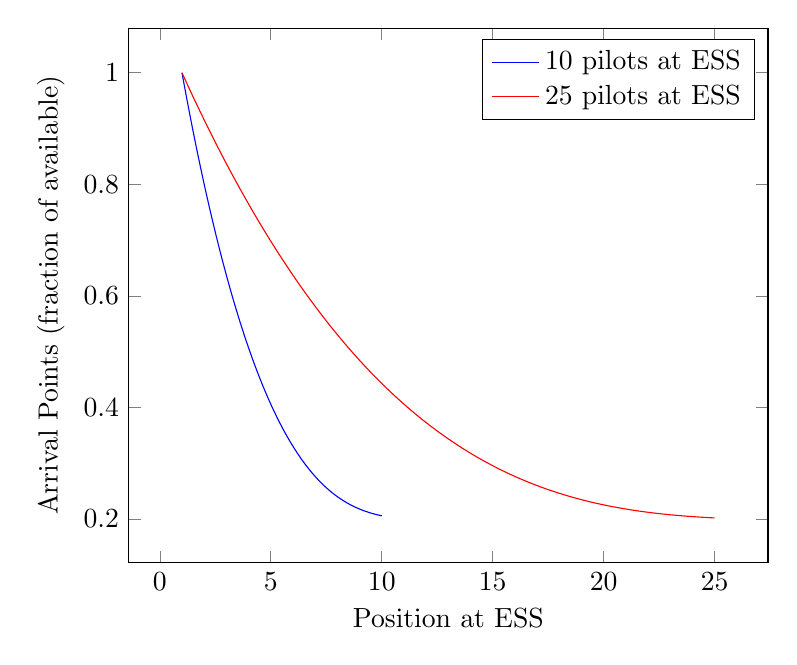
\begin{tikzpicture}
\begin{axis}[ xlabel=Position at ESS
            , ylabel=Arrival Points (fraction of available)
            , width=0.8\textwidth
            ]
    \addplot[ blue
            , domain=1:10
            , samples=100
            ]{0.2 + 0.037*(1 - (x - 1)/10) + 0.13*(1 - (x - 1)/10)^2 + 0.633*(1 - (x - 1)/10)^3};
    \addplot[ red
            , domain=1:25
            , samples=100
            ]{0.2 + 0.037*(1 - (x - 1)/25) + 0.13*(1 - (x - 1)/25)^2 + 0.633*(1 - (x - 1)/25)^3};
    \legend{10 pilots at ESS, 25 pilots at ESS} 
\end{axis}
\end{tikzpicture}

    \caption{Sample arrival points distributions}
\end{figure}

\begin{pg}
No arrival points are awarded in Paragliding.
\end{pg}
\end{document}
